\documentclass[border=4pt]{standalone}
% Shared preamble + reusable TikZ styles for every figure in this directory.
% Each figure \input's this right after its \documentclass. The leading
% underscore marks it as a partial: buildFigures skips underscore-prefixed files
% (this is not a standalone document of its own).

\usepackage{tikz}
\usepackage{xcolor}
\usepackage{fontspec}
\usetikzlibrary{calc, arrows.meta}

% Match the document: Poppins (vendored in figures/fonts/, loaded by path so the
% build is self-contained). Compiled with lualatex.
\setsansfont{Poppins}[
  Path = figures/fonts/, Extension = .ttf,
  UprightFont = *-Regular, ItalicFont = *-Italic,
  BoldFont = *-SemiBold, BoldItalicFont = *-SemiBoldItalic]
\renewcommand\familydefault{\sfdefault}

% IBM Plex Mono — the site's code font. Figure labels are Lean identifiers
% (Point, Line, LiesOn, A, ℓ), so we set them in the code font to match the
% rendered code (and Plex Mono has the ℓ glyph that Poppins lacks).
\newfontfamily\figmono{IBMPlexMono}[
  Path = figures/fonts/, Extension = .otf,
  UprightFont = *-Regular, ItalicFont = *-Italic,
  BoldFont = *-SemiBold, BoldItalicFont = *-SemiBoldItalic]

% Brand palette — kept in step with the site CSS (--canva-purple / --canva-ink).
\definecolor{canvapurple}{HTML}{6A21CC}
\definecolor{canvaink}{HTML}{15171C}
% Dark teal for geometric lines — stands out against the purple labels.
\definecolor{canvateal}{HTML}{0E7490}
% Inline-code "chip" look, matching the prose's inline code (CSS: bg #f3effe,
% text #6420c9, rounded corners).
\definecolor{canvachipbg}{HTML}{F3EFFE}
\definecolor{canvachipink}{HTML}{6420C9}

% Reusable TikZ styles:
%   geoline  — a geometric line (dark-teal stroke)
%   point    — a point (filled ink dot); place with \node[point] at (..) {};
%   ptlabel  — a name for a point/line (A, B, C, ℓ, m, n) in the code font
%   concept  — a purple annotation naming a concept (Point, Line, …), code font
%   leader   — a thin arrow from an annotation to the thing it points at
\tikzset{
  geoline/.style = {canvateal, line width=2pt},
  point/.style   = {canvaink, circle, fill, inner sep=0pt, minimum size=8pt},
  ptlabel/.style = {canvaink, font=\figmono\fontsize{12}{15}\selectfont},
  concept/.style = {canvapurple, font=\figmono\fontsize{11}{13}\selectfont},
  leader/.style  = {canvaink, line width=1pt, -{Stealth[length=8pt]}},
  % namechip — a Lean identifier on a rounded light-purple chip, mirroring the
  % prose's inline-code styling (Plex Mono, purple text on a light-purple fill).
  namechip/.style = {text=canvachipink, fill=canvachipbg, rounded corners=3pt,
                     inner xsep=5pt, inner ysep=3pt, font=\figmono\fontsize{12}{15}\selectfont},
}


\begin{document}
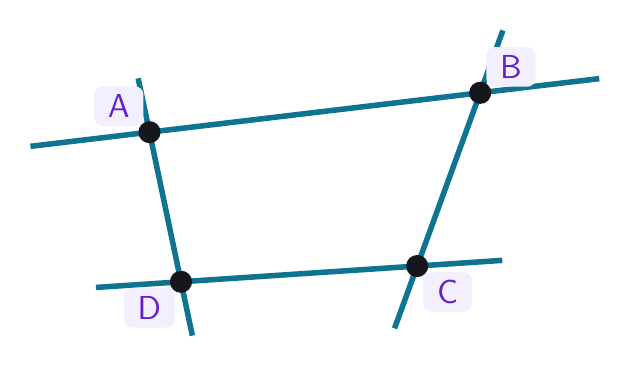
\begin{tikzpicture}
  % Four points in general position — an irregular quadrilateral, no three
  % collinear.
  \coordinate (A) at (1.0,2.4);
  \coordinate (B) at (5.2,2.9);
  \coordinate (C) at (4.4,0.7);
  \coordinate (D) at (1.4,0.5);

  % The four lines through adjacent pairs, each extended a little past both
  % points (lines don't terminate). The extension is kept short so the lines
  % don't reach each other's crossings outside the quad.
  \draw[geoline] ($(A)!-0.36!(B)$) -- ($(A)!1.36!(B)$);
  \draw[geoline] ($(B)!-0.36!(C)$) -- ($(B)!1.36!(C)$);
  \draw[geoline] ($(C)!-0.36!(D)$) -- ($(C)!1.36!(D)$);
  \draw[geoline] ($(D)!-0.36!(A)$) -- ($(D)!1.36!(A)$);

  % The four points, labelled outward from the centre.
  \node[point] at (A) {}; \node[namechip, above left=2pt]  at (A) {A};
  \node[point] at (B) {}; \node[namechip, above right=2pt] at (B) {B};
  \node[point] at (C) {}; \node[namechip, below right=2pt] at (C) {C};
  \node[point] at (D) {}; \node[namechip, below left=2pt]  at (D) {D};
\end{tikzpicture}
\end{document}
